\documentclass[12pt]{article}

\usepackage[margin=1in]{geometry}
\usepackage{amsmath,amsthm,amssymb}
\usepackage{mathtools}
\usepackage{mathrsfs}
\usepackage{enumitem}
\usepackage{physics}
\usepackage{empheq}
\usepackage{float}
\usepackage{graphicx}
\graphicspath{ {./images/} }

\usepackage{tikz}
\usetikzlibrary{calc,decorations.markings,patterns}

\newcommand{\magsq}[1]{\big|#1\big|^2}
\newcommand{\avg}[1]{\left<#1\right>}
\newcommand{\fullint}{\int_{-\infty}^\infty}
\newcommand{\fullintd}[1]{\fullint\dd#1\:}
\newcommand{\cint}[2]{\int_{#1}^{#2}}
\newcommand{\cintd}[3]{\cint{#1}{#2}\dd#3\:}

\begin{document}

\title{Midterm}
\author{Phys 611}
\date{Due: Thursday, October 27, 2022}
\maketitle

\section*{Problem 1}
\begin{figure}[H]
    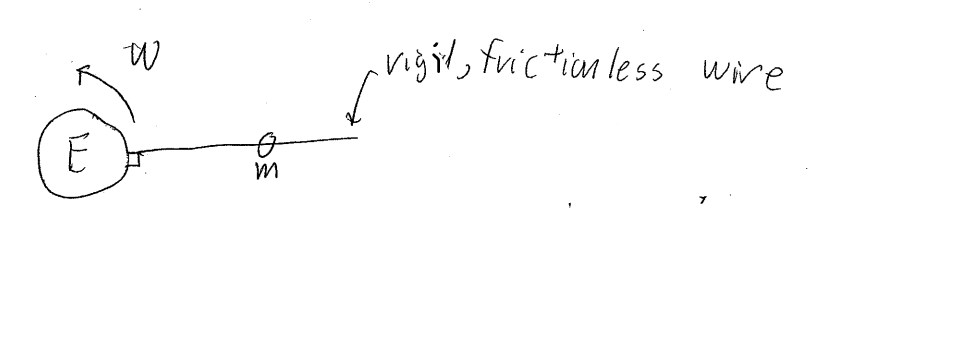
\includegraphics{Problem1}
    \centering
\end{figure}
A rigid, frictionless wire is attached vertically to the surface of the Earth (which, I remind you, is rotating). A bead of mass $m$ slides frictionlessly on this wire.
\begin{enumerate}[label=(\alph*)]
    \item Write down the Lagrangian for the mass $m$. Express you answer entirely in terms of the radius $R$ of the Earth, its angular frequency of rotation $\omega$, and the acceleration due to gravity at the surface of the Earth, as well as, of course, whatever coordinates you choose as variables of your Lagrangian, and the mass $m$ of the bead.
    \item Find a constant of the mortion of the bead. Is the bead's energy conserved?
    \item Is there a point on the wire at which, in principle, the bead can sit forever, moving neither in nor out? If so, how far is it from the center of the Earth? Give a numerical answer, using the known values of $g$, $\omega$, and $R$ for the Earth.
    \item Suppose the bead starts \textit{just} below (i.e. closer to Earth) than the point found in 1c), and is initially stationary with respect to the wire. Describe its subsequent motion. Will it hit the ground? If it does, how fast is it moving when it does?
    \item Same as 1d), but now the bead starts at rest relative to the wire at a point just \textit{above} the point found in 1c). Now describe its subsequent motion.
    \item Suppose the wire ends a distance $r_e$ from the center of the Earth. Find the \textit{smallest} value of $r_e$ such that, once the bead flies off the end of the wire, it escapes from the earth. Assume the same initial conditions as in 1e. \\ 
        For an \textit{arbitrary} $r_e$ (not necessarily the one you've just found) find the shape of the orbit $r(\theta)$ of the bead \textit{after} it comes off the wire. Express your answer entirely in terms of $R$, $g$, $\omega$, and $r_e$.
\end{enumerate}


\section*{Problem 2}
\begin{figure}[H]
    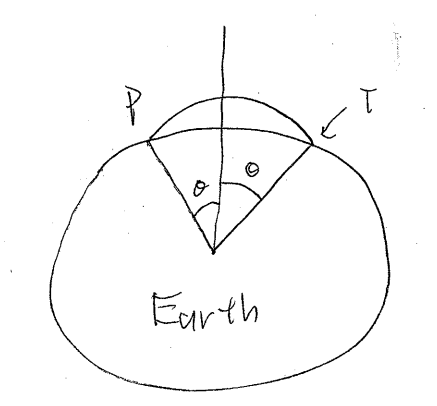
\includegraphics{Problem2}
    \centering
\end{figure}
Consider the problem of launching a projectile (e.g. a Scud missle) from one point $P$ on the Earth's surface to another point $T$ an angle $2\theta$ away as measured from the Earth's center. Treat the Earth as spherically symmetric and ignore its rotation.
\begin{enumerate}[label=(\alph*)]
    \item At what angle $\phi$ to the vertical should the projectile be launched so as to minimize the launch speed $v_0$ required to get it to $T$?
    \item What launch speed $v_0$ \textit{is} required if we launch at that angle? Express your answer in terms of $g$ and $R$.
    \item For $\theta = 45^{\circ}$, how long is the projectile in flight? Give a numerical answer using the known values of $g$ and $R$.
\end{enumerate}


\section*{Problem 3}
\begin{figure}[H]
    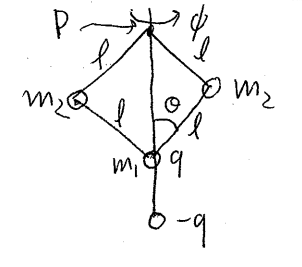
\includegraphics{Problem3}
    \centering
\end{figure}
Consider a device similar to that in problem set \#2, with 3 masses connected by rigid rods of length $l$ to each other and to a pivot $P$. The mass $m_1$ is, as before, constrained to slide on a vertical shaft, and the rods are constrained to remain coplaner. There is no longer any gravity, but the mass $m_1$ carries a charge $q$. A charge $-q$ is \underline{fixed} to the shaft in a position such that, when $\theta = 0$, the mass $m_1$ \textit{just} touches it.\\
Everything else in the figure is unchanged, and there are no other forces in the problem other than those enforcing the constraints. The entire apparatus is free to rotate about the shaft, which is fixed.
\begin{enumerate}[label=(\alph*)]
    \item Write down the Lagrangian for this system.
    \item Find 2 independent conserved quantities.
    \item Suppose initially $\theta > 0$ and the entire apparatus is rotating around the shaft with angular speed $\omega$. Show that, if $\omega$ exceeds some critical value $\omega_c$, the mass \underline{never} touches the fixed $-q$ charge, and calculate $\omega_c$ in terms of $q$, $l$, $m_1$, and $m_2$.
\end{enumerate}



\section*{Problem 4}
Consider central force motion in the potential
\begin{equation}
    U(r) = -\frac{\mu}{r} + \frac{k}{r^2}
\end{equation}
Note: $k$ need \underline{not} be $>0$. \\ \\
An object of mass $m$ moving in this potential is observed to move in an orbit of the following shape: \\
\begin{figure}[H]
    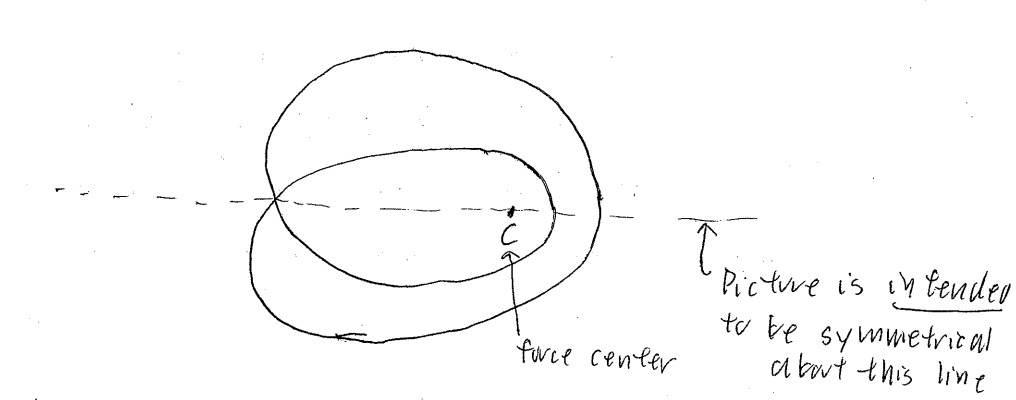
\includegraphics{Problem4}
    \centering
\end{figure}
Calculate the angular momentum per unit mass $h$ of the object. Express your answer entirely in terms of $\mu$, $k$, and $m$.

\section*{Problem 5}
\begin{figure}[H]
    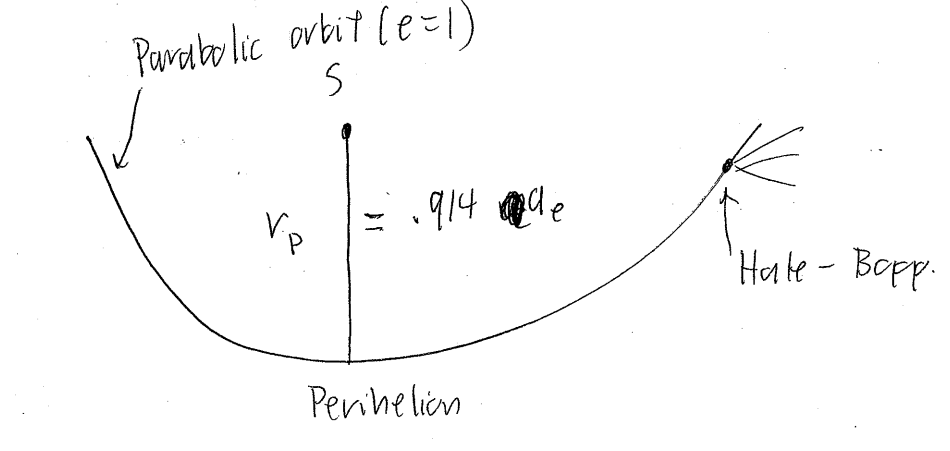
\includegraphics{Problem5}
    \centering
\end{figure}
The comet Hale-Bopp made its closest approach to the sun (a distance of 0.914 $a_e$, where $a_e$ is the semi-major axis of the Earth's orbit) on April 1, 1997. We'd like to know how far away from the sun it was on April 1, 1998. It's orbit is, to a good approximation, parabolic (i.e., the eccentricity $e$ of the orbit is very nearly 1).
\begin{enumerate}[label=(\alph*)]
    \item Calulate $t(r)$, defining $t=0$ to be the time of perihelion. Express your answer in terms of the period $T$ of a circular orbit of radius $r_p$. (I.e., write $t=Tf(r)$, and find $f(r)$).
    \item Invert your answer to a) to find $r(t)$, and numerically evaluate this to find the distance of Hale-Bopp from the sun on April 1, 1998. You may express your answer as a numerical constant times $a_e$, but you must give the numerical value of the numerical constant. (Hint: to solve $x^3 + 3x = y$, try the substitution $x = u - \frac{1}{u}$).
\end{enumerate}

\end{document}